\documentclass[12pt]{article}
\usepackage[top=1cm, bottom=2cm, right=1cm, left=1cm]{geometry}
\usepackage{amsfonts, amssymb, amsmath, hyperref}
\usepackage{graphicx}
\usepackage[T1, T2A]{fontenc}% T2A for Cyrillic font encoding
\usepackage[english, russian]{babel}
\usepackage[justification=centering]{caption}
\usepackage{wrapfig,lipsum,booktabs}
\usepackage{placeins}
\usepackage{subcaption}
\usepackage{multirow}
\usepackage{longtable}

\begin{document}
\title{\textbf{Лабораторная работа 3.2.5}\\ [2pt]{Свободные и вынужденные
колебания в электрическом контуре}}
\date{\today}
\author{Татаурова Юлия Романовна}

\begin{document}
\maketitle
\textbf{Цель работы:} исследование свободных и вынужденных колебаний в
колебательном контуре.\\\indent
\textbf{Оборудование:} осциллограф, генератор сигналов, магазин сопротивления, магазин емкости, магазин индуктивности, соединительная коробка с шунтирующей емкостью, соединительные одножильные и коаксиальные провода.

\section*{Экспериментальные данные}

\begin{figure}[h!]
    \centering
    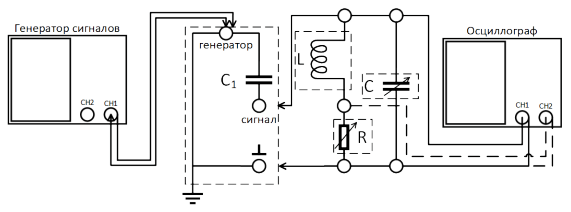
\includegraphics[width=12cm]{images/setup.png}
    \caption{Схема установки вынужденных колебаний}
\end{figure}
\indent Генератор подает на вход периодические короткие импульсы, которые заряжают конденсатор $C$. За время между импульсами конденсатор разряжается через резистор и катушку.

\subsection*{Измерение периодов свободных колебаний}

\begin{table}[h!]
    \begin{minipage}{0.4\linewidth}
        \centering
        \begin{tabular}{|c|c|c|}
            \hline
            $L$, мГн  & $T$, мкс & $C_0 = \frac{T^2}{2\pi^2 L}$, нФ\\\hline
            100     & $69.0 \pm 0.1$ & $1.206 \pm 0.005$\\\hline
        \end{tabular}
        \caption{Начальные данные}
    \end{minipage}
    \hfill
    \begin{minipage}{0.7\linewidth}
        \centering
        \begin{tabular}{|c|c|c|c|c|c|c|c|}
            \hline
            $C$, нФ  & 0& 1& 3& 5& 6& 8& 9\\\hline
            $T$, мкс & 69& 94& 132& 158& 168& 188& 200 \\\hline
        \end{tabular}
        \caption{Зависимость периода колебаний от емкости $T(C)$}
    \end{minipage}
\end{table}
\newpage

\begin{figure}[h!]
\begin{subfigure}{0.45\linewidth}
    \centering
    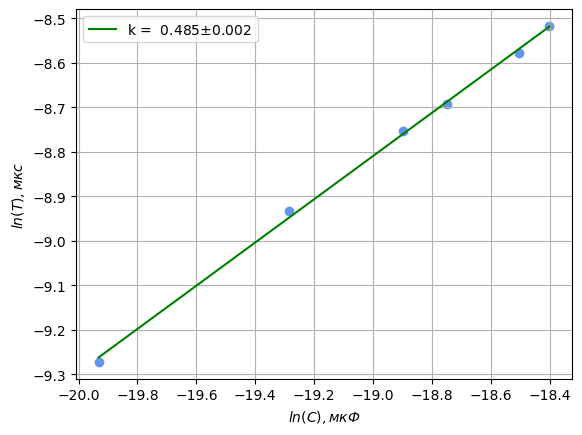
\includegraphics[width=9cm]{images/plot1.png}
    \caption{График зависимости $T(C)$}
\end{subfigure}
\hfill
\begin{subfigure}{0.55\linewidth}
    \centering
    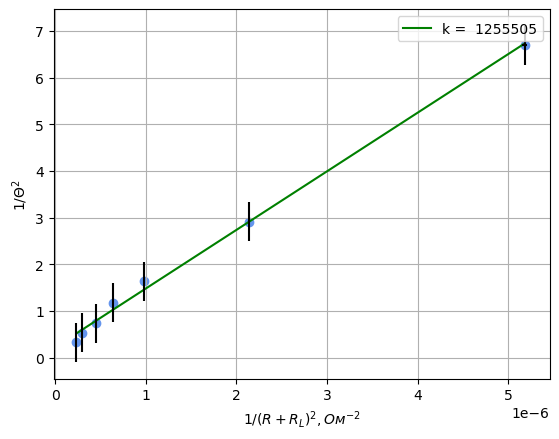
\includegraphics[width=9cm]{images/plot2.png}
\caption{График зависимости $Y = 1 / \Theta^2 \text{ от } X = 1 /  (R + R_L)^2$}
\end{subfigure}
\end{figure}
\indent График $T(C)$ был построен с учетом $C_0$ и него видно, что $T \propto \sqrt{C}$.

\subsection*{Критическое сопротивление и декремент затухания}
\indent $\nu_0 = 6.5$ кГц; $C^{*} = \left (\frac{1}{2\pi \nu_0}\right ) ^ 2 \cdot \frac{1}{L} = 6.00 \pm 0.01$ нФ
$R_{\text{cr}} = 2\sqrt{\frac{L}{C^{*}}} = 8168 \pm 23$ Ом. \\
\indent Меняя сопротивление $R$, мы определили при каком значении колебательный режим переходит в апериодический: $R \approx 6$ кОм.\\\indent 
Логарифмический декремент затухания $\Theta$ можно найти по формуле:
\begin{equation}
    \Theta = \frac{1}{n}\ln\left (\frac{U_{\text{m}}}{U_{\text{m+n}}}\right )
\end{equation}
\begin{align}
    \frac{\pi}{\Theta} = \frac{\pi}{\gamma T_1} = \frac{1}{2}\sqrt{\frac{R_{\text{cr}}^2}{R^2} - 1} \Rightarrow\\
    \frac{1}{\Theta^2} = \frac{1}{4\pi^2}\left ( \frac{R_{\text{cr}}^2}{R^2} - 1 \right ) \Rightarrow k = \frac{R_{\text{cr}}^2}{4\pi^2}
\end{align}
\begin{table}[h!]
    \centering
    \begin{tabular}{|c|c|c|c|c|c|c|c|}
        \hline
        $R$, Ом & 408 & 653 & 980 & 1225 & 1470 & 1796 & 2041\\\hline
        $\Theta$(п.2.3) ($\varepsilon\approx 6\%$)& 0.39& 0.59& 0.78& 0.92& 1.17& 1.37& 1.76\\\hline
        $\Theta$(п.2.4) ($\varepsilon\approx 25\%$)& 0.26& 0.31& 0.39& 0.55& 0.66& 0.85& 0.97\\\hline
        $Q$ (п.2.3) &8.1& 5.4& 4.0& 3.4& 2.7& 2.3& 1.8\\\hline
        $Q$(п.2.4) &12.3& 10.1& 8.0& 5.7& 4.8& 3.7& 3.2\\\hline
    \end{tabular}
    \caption{Зависимость декремента затухания от сопротивления}
\end{table}
\\
\indent $R_{\text{cr}} = 2\pi\sqrt{\frac{\Delta Y}{\Delta X}} = 7040 \pm 440$ Ом ($\varepsilon \approx 6\%$)

\subsection*{Свободные колебания на фазовой плоскости}
Теперь подадим на второй канал осциллографа падение напряжения с резистра. Все данные представлены в таблице 3.
\newpage
\begin{figure}[h!]
    \begin{subfigure}{0.43\linewidth}
    \centering
    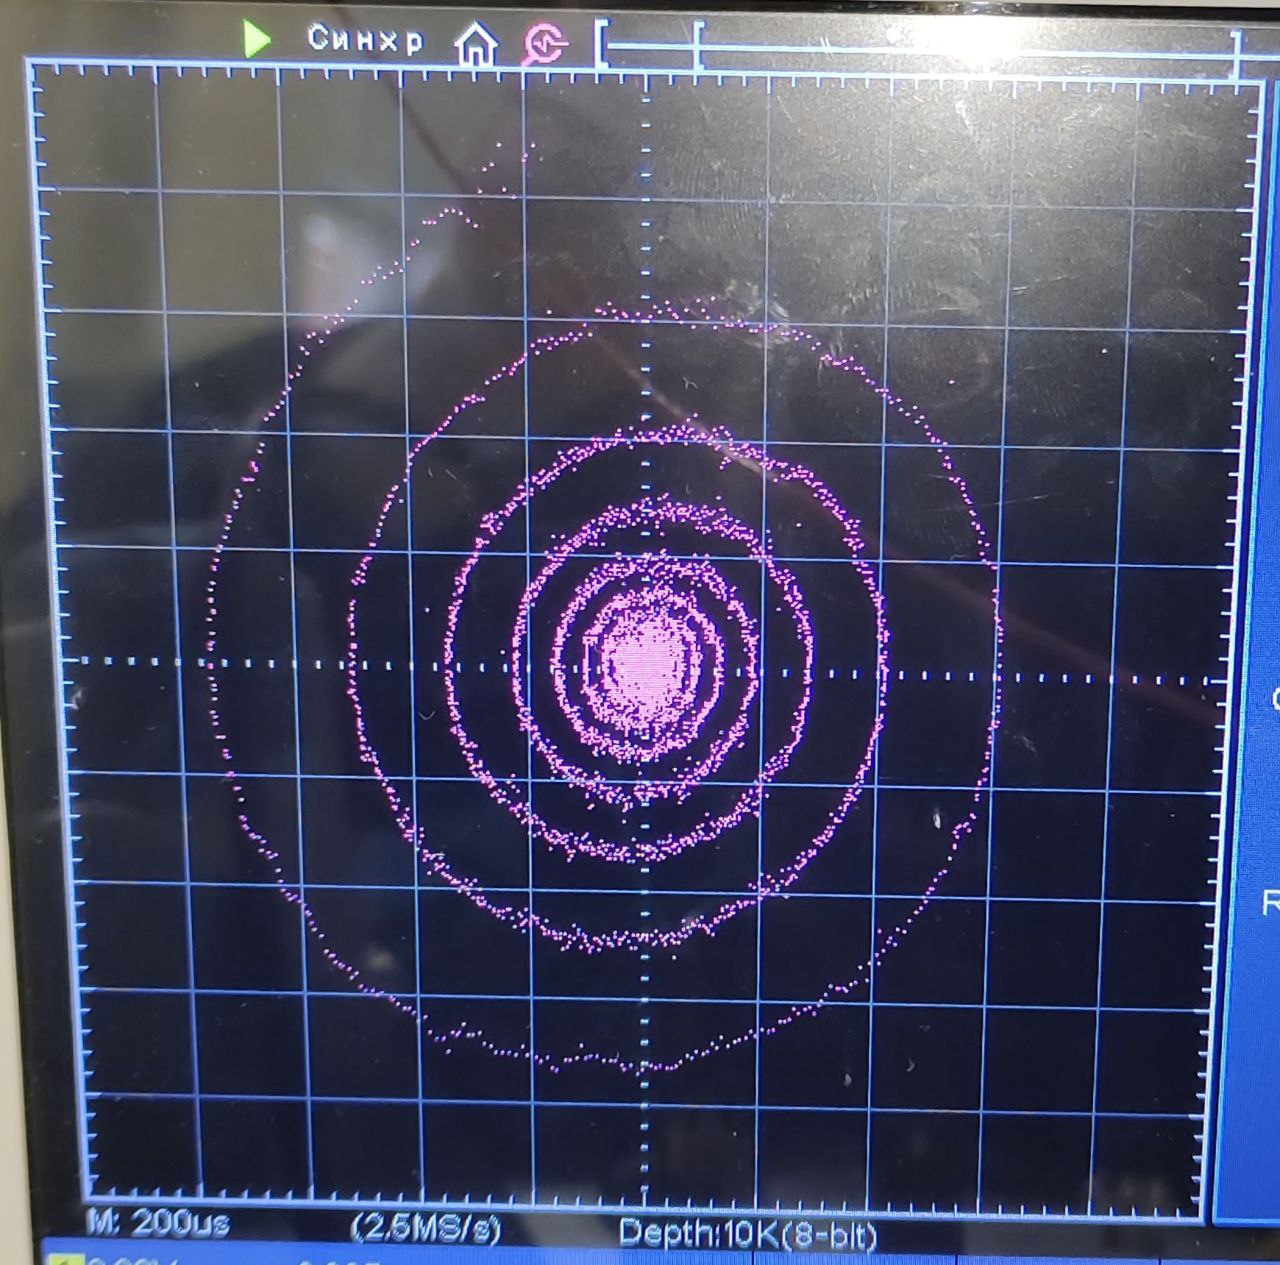
\includegraphics[width=8cm]{images/spiral.jpg}
    \caption{Наблюдение затухающих колебаний на фазовой плоскости}
    \end{subfigure}
    \hfill
    \begin{subfigure}{0.55\linewidth}
    \centering
    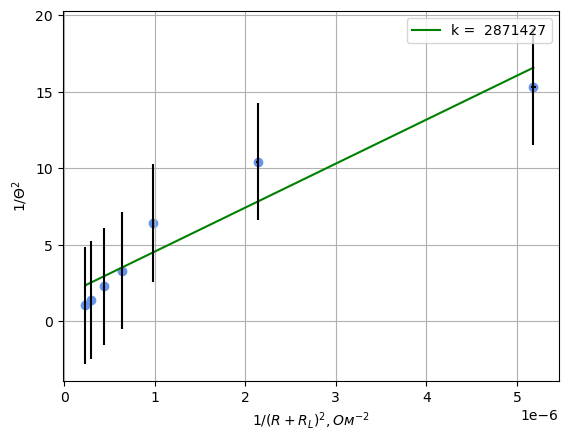
\includegraphics[width=8cm]{images/plot3.png}
    \caption{График зависимости $Y = 1 / \Theta^2 \text{ от } X = 1 /  (R + R_L)^2$}
    \end{subfigure}
\end{figure}

\subsection*{Исследование резонансных кривых}

$C = C^{*}$ = 6 нФ; $R_1$ = 408 Ом; $R_2$ = 2042 Ом

\begin{figure}[h!]
        \centering
    \begin{subfigure}{0.42\linewidth}
        \centering
        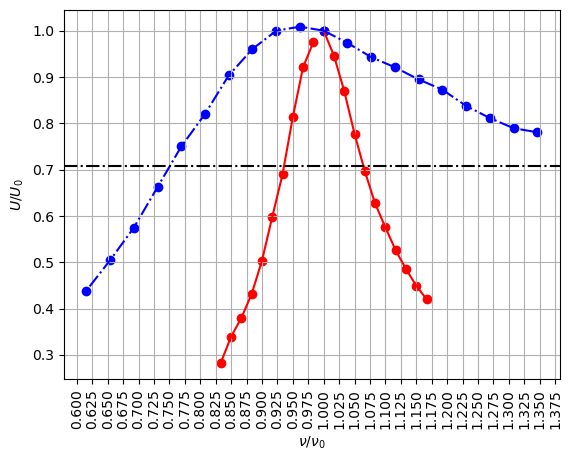
\includegraphics[width=10cm]{images/plot4_R1_A.png}
        \caption{АЧХ при $R_1 = 408$ Ом и $R_2 = 2042$ Ом}
    \end{subfigure}
    \hfill
    \begin{subfigure}{0.47\linewidth}
        \centering
        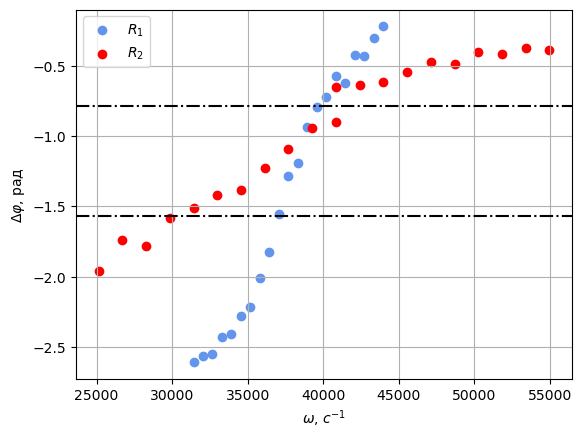
\includegraphics[width=10cm]{images/plot5_R1_P.png}
        \caption{ФЧХ при $R_1 = 408$ Ом и $R_2 = 2042$ Ом}
    \end{subfigure}
\end{figure}
Определим добротность контура по АЧХ по формуле $Q = \frac{\omega_0}{\Delta\Omega}$ $\Rightarrow$\\\indent $Q_1 = 7.6 \pm 1.0 (\approx 12\%)$ и $Q_2 = \frac{\omega_0}{\Delta\Omega} = 2.4 \pm 0.3 (\approx 12\%)$.

\newpage

\begin{figure}[h!]
\begin{minipage}{0.45\linewidth}
    \centering
    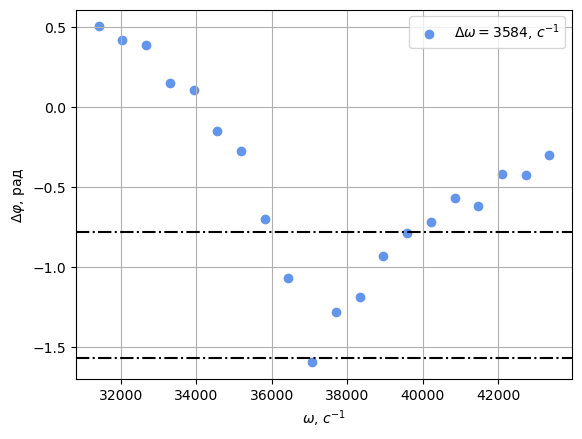
\includegraphics[width=8cm]{images/plot6.png}
    \caption{Определение добротности по ФЧХ($R_1$)}
\end{minipage}
\hfill
\begin{minipage}{0.49\linewidth}
{
Теперь определим добротность контура по ФЧХ по формуле $Q = \frac{\omega_0}{\Delta\omega}$, где 
$\Delta\omega$ - расзность частот на уровнях $-\pi/2 \text{ и }-\pi/4$. \\
$Q_1 = 10.5 \pm 0.7 (\approx 7\%)$.\\
\indent $Q_2$ таким способом не получается определить, т.к количества точек недостаточно.\\
}


    \centering
    \begin{tabular}{|c|c|c|}
            \hline
            $\Theta\text{/}R$ & $R_1$ & $R_2$ \\\hline
            По нарастанию & $0.38 \pm 0.03 (8\%)$ & $1.45 \pm 0.06 (4\%)$\\\hline
            По затуханию & $0.26 \pm 0.04 (15\%)$ & $1.69$\\\hline
    \end{tabular}
    \caption{Определение декремента затухания по нарастанию и затуханию}
\end{minipage}
\end{figure}
% Теперь определим добротность контура по ФЧХ по формуле $Q = \frac{\omega_0}{\Delta\omega}$, где 
% $\Delta\omega$ - расзность частот на уровнях $-\pi/2 \text{ и }-\pi/4$. \\
% $Q_1 = 10.5 \pm 0.7 (\approx 7\%)$.\\ 
% \indent $Q_2$ таким способом не получается определить, т.к количества точек недостаточно.\\\\\\\\\\\\\\\\\\
%
\subsection*{Процессы установления и затухания}

\indent $R = R_1$ = 408 Ом; $\nu$ = 6 кГц; $\tau = 20$ мс; $N$ = 15\\ 
\indent Декремент затухания по скорости нарастаниявычисляется по формуле:
\begin{equation}
    \Theta = \frac{1}{n}\ln\frac{U_0 - U_k}{U_0 - U_{k + n}}
\end{equation}
\indent Декремент затухания колебательной системы по скорости затухания вычисляется по формуле (1).

\section*{Результаты и выводы}

\begin{table}[h!]
    \centering
    \begin{tabular}{c|c|c|c|c|c|c|c|}
        \hline
        \multirow{2}{*}{$R$} & \multicolumn{3}{|c|}{Свободные колебания} & \multicolumn{4}{|c|}{Вынужденные колебания}\\
         & $f(L, C, R)$ & $f(\Theta)$ & Спираль & АЧХ & ФЧХ & Нарастание & Затухание\\\hline
        $R_1 = 408$ Ом & 8.47($0.6\%$) & $8.1\pm 0.5$ & $12.3\pm 3.0 $ & $7.6\pm1.0$ & $10.5\pm0.7$ & $8.3\pm 0.7$ & $12.0\pm1.8$\\\hline
        $R_2 = 2042$ Ом & 1.72($0.6\%$) & $1.8\pm 0.1$ & $3.2\pm 0.8$ & $2.4\pm0.3$ & - & $2.7\pm 0.1$ & 1.9\\\hline
    \end{tabular}
    \caption{Сравнение результатов вычисления добротности разными способами}
\end{table}

1) Определили зависимость периода свободных колебаний от емкости конденсатора: $T \propto \sqrt{C}$\\
\indent2) Определили зависимость логарифмического декремента затухания от сопротивления: $\Theta \propto R$. 
И из этого нашли критическое сопротивление $R_{\text{cr}} = 7040\pm440$ Ом. Вычисленное формульное значение $R_{\text{cr}} = 8168\pm23$ Ом. Однако апериодический режим наблюдался уже при 6 кОм.\\
\indent 3)Рассмотрели свободные колебания на фазовой плоскости. На экране осциллографа наблюдалась спираль, что как раз и соответствует теории для затухающий колебаний. \\
\indent 4)Исследовали резонансные кривые, строили для них АЧХ и ФЧХ. По ним определили добротность контура.\\
\indent 5)Исследовали процессы установления и затухания. По ним так же определили добротность контура.




\end{document}
